\documentclass[pdf]{beamer}
\mode<presentation>{}
\usetheme{Dresden}
\usepackage{apalike}
\usepackage{graphicx}
\usepackage{mwe,tikz}\usepackage[percent]{overpic}
%% preamble
\title{Undular Bores of the Serre Equations}
\author{Jordan Pitt, Stephen Roberts and Christopher Zoppou \\ Australian National University}
\newcommand\solidrule[1][0.25cm]{\rule[0.5ex]{#1}{1pt}}
\newcommand\dashedrule{\mbox{\solidrule[2mm]\hspace{2mm}\solidrule[2mm]}}
\newcommand{\dotrule}[1]{%
	\parbox[]{#1}{\dotfill}}

\begin{document}
%% title frame
\begin{frame}
\titlepage
\end{frame}
%% normal frame
\section{Undular Bores}
\subsection{Introduction}
\begin{frame}{Undular Bores}
	%undular bores occur in many physical systems from tidal bores, tsunamis to plasma dynamics, using these equations we are most interested in tidal bores and tsunamis but understanding bores here can give insight into plasma dynamics due to the similarity of terms
	
	%the main mechanic behind undular bores is dispersion where waves of different frequencies are dispersed due to their different wave speeds, without which such phenomenon would appear as a single advnacing shock front as in the SWWE
	
	%such phenomenon are hard to understand analytically, and for the equations of interest there are no analytic solutions and few insights into how undular bores should behave
	
	\begin{figure}
		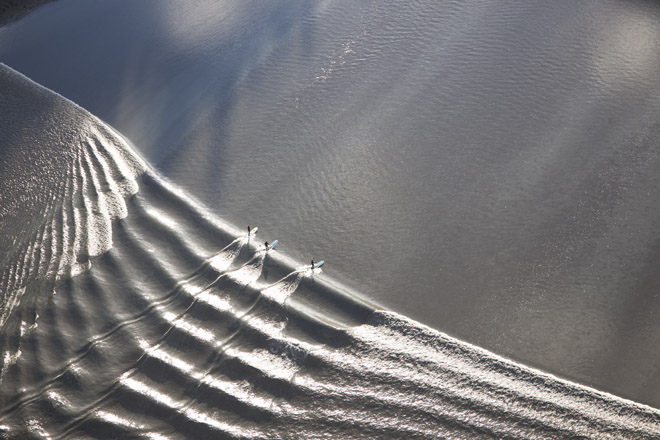
\includegraphics[width=6cm]{../Pics/Web/tidal.jpg}
		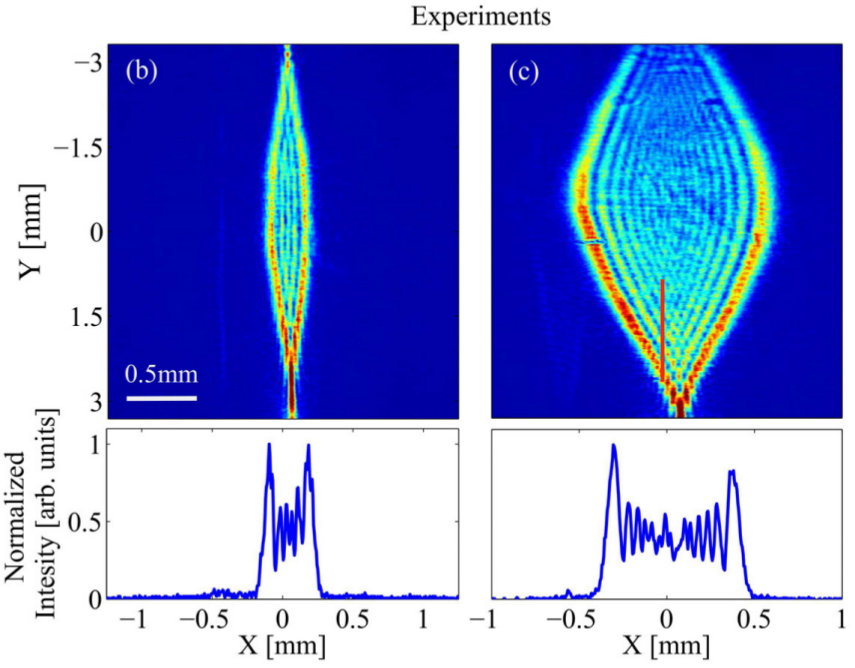
\includegraphics[width=5.5cm]{../Pics/Web/U1.png}
		\caption{examples of undular bores from tidal flows to even optics.}
		\label{fig:RLpics}
	\end{figure}
	
\end{frame}

\begin{frame}{Dam Break}
 %We are going to study undular bores by looking at the dam break problem, where we have two different still bodies of water seperated by a dam wall and then at $t=0$ the dam wall is removed
 Fluid depth ($h$) :
 \begin{subequations}
 	\begin{gather*}
 h(x,0) = \left\lbrace \begin{array}{c c}
 h_1  & x \le x_0\\ h_0  & x > x_0 
 \end{array} \right. 
 	\end{gather*}
 Fluid velocity  ($u$) :
 	\begin{gather*}
 	u(x,0) = 0.0 .
 	\end{gather*}
 \end{subequations} 
  
	
\end{frame}

\begin{frame}{Smoothing}

	
	\begin{figure}
		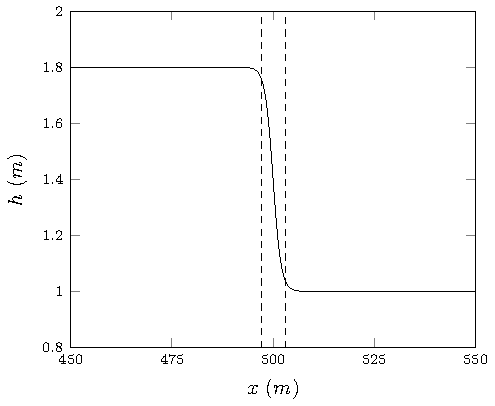
\includegraphics[width=6cm]{../Pics/Edit/ICbetaexample.pdf}
		\caption{Example of water profile of a smoothed dam break with a transition width $\beta$ of $5.8888$.}
	\end{figure}
	
\end{frame}

\begin{frame}{Serre Equations}
	
	%The Serre equations, also known as the Su Gardner or Green-Naghdi equations in 1D like the SWWE are a depth averaged approximation to the Euler Equations for incompressible fluids
	%The result of this is that we basically get some modification to the SWWE, which is a result of assuming a linear vertical velocity profile, rather and a zero vertical velocity throughout the depth. This assumption generates the dispersion terms which allow us to model dispersion and undular bores and as noted in the literature this form of dispersion applies outside the standard fluid dynamics (such as plasma)
	%these equations are also considered a very good model for fluid dyanmics up to wave breaking
	\begin{subequations}\label{eq:Serre_conservative_form}
		\begin{gather*}
		\dfrac{\partial h}{\partial t} + \dfrac{\partial (uh)}{\partial x} = 0,
		\label{eq:Serre_continuity}
		\end{gather*}
		\begin{gather*}
		\underbrace{\underbrace{\dfrac{\partial (uh)}{\partial t} + \dfrac{\partial}{\partial x} \left ( u^2h + \dfrac{gh^2}{2}\right )}_{\text{Shallow Water Wave Equations}} + \underbrace{\dfrac{\partial}{\partial x} \left (  \dfrac{h^3}{3} \left [ \dfrac{\partial u }{\partial x} \dfrac{\partial u}{\partial x} -u \dfrac{\partial^2 u}{\partial x^2}  - \dfrac{\partial^2 u}{\partial x \partial t}\right ] \right )}_{\text{Dispersion Terms}} = 0}_{\text{Serre Equations}}
		\label{eq:Serre_momentum}
		\end{gather*}
	\end{subequations}
\end{frame}

\section{Literature Results}
\subsection{Numerical}
\begin{frame}{Literature Results}
	%Numerical method qas quite rudimentary, and was basically two second order finite difference approximations (lax wendroff for mass, and naive for momentum)
	%actually requires some smoothing of the problem.
\begin{figure}
	\centering
	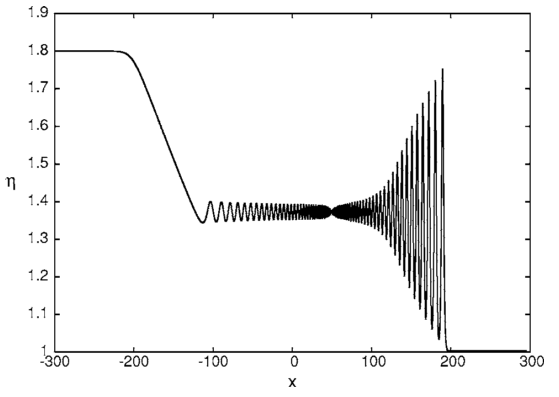
\includegraphics[width=7cm]{../Pics/Lit/SmoothDBEl.png}
	\caption{Fluid depth at $150s$ obtained from numerical method by El and Grimshaw \cite{El-etal-2006}.}
	\label{fig:ElDB}
\end{figure}	
\end{frame}

\begin{frame}{}
	%Numerical method made use of a reformulation of the equations to get a conservation form of the Serre equations with an additional elliptic equation to solve. It then used a first order Gudonov type FVM technique on the conservative form, and a second order naive finite difference scheme on the elliptic equation. 
	\begin{figure}
		\centering
		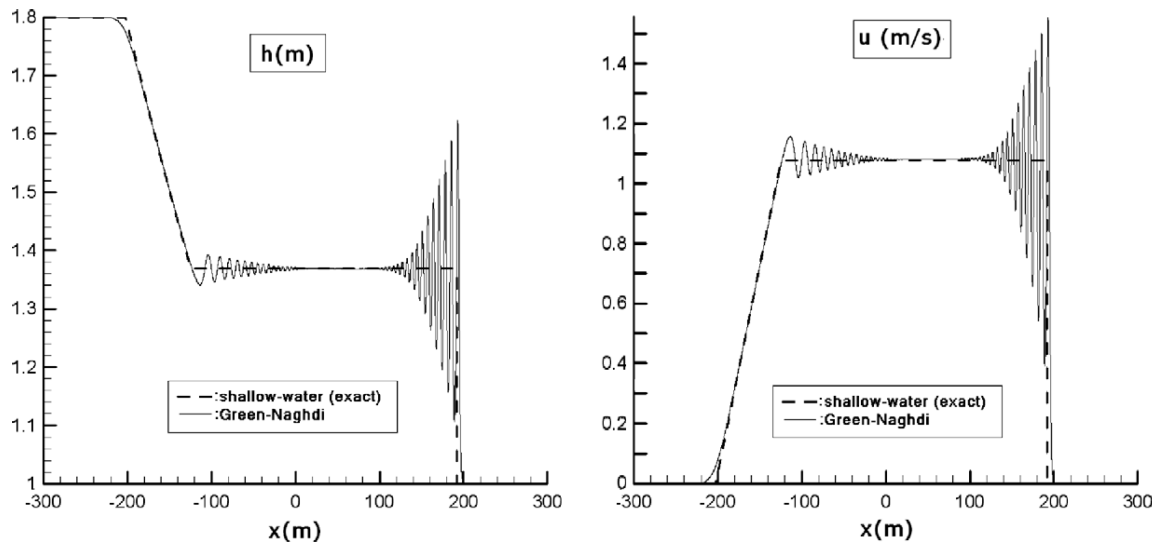
\includegraphics[width=9cm]{../Pics/Lit/DBhank.png}
		\caption{Fluid depth at $48s$ obtained from numerical method by Le M\'{e}tayer \cite{Hank-etal-2010-2034} (The Serre equations are also known as the Green Naghdi equations).}
		\label{fig:HankDB}
	\end{figure}	
\end{frame}

\begin{frame}{}
	%Numerical Method uses a fourth order Galerkin FEM scheme with 4th order RK steps on a smoothed dam break problem (alpha = 0.5, quite slow transition)
	
	%both of these papers claim to refute the results of Els numerical method, and appear to demonstrate that indeed our solution should have oscialltions both near the rearefaction fan and the shock with a constant state between the two. So we should resolve this conflict
	\begin{figure}
		\centering
		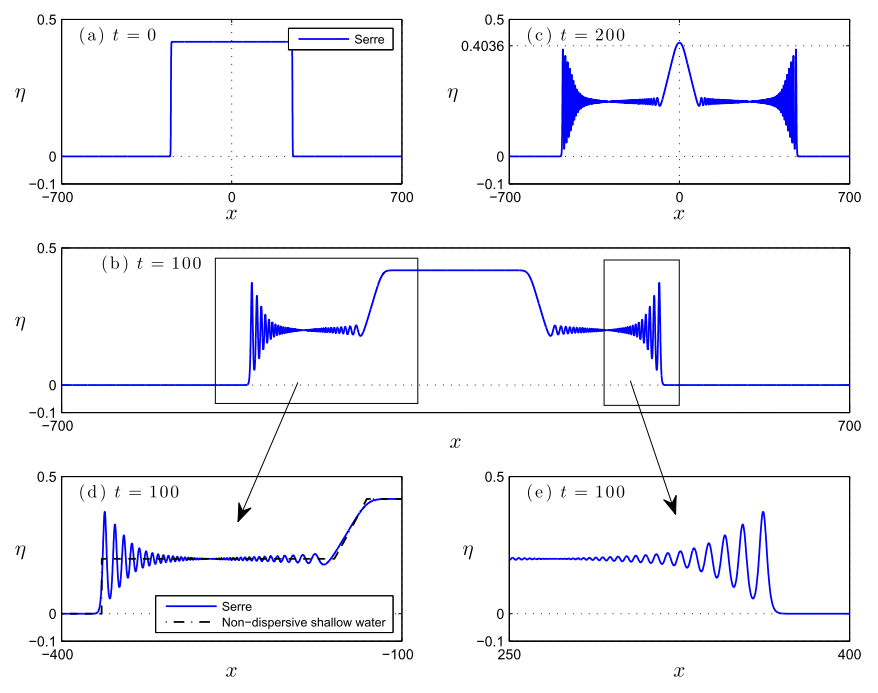
\includegraphics[width=7cm]{../Pics/Lit/SmoothDBDutyhk.png}
		\caption{Wave height at various times for the smoothed dam break problem obtained from numerical method by Mitsotakis \cite{Mitsotakis-etal-2014}.}
		\label{fig:DuthykDB}
	\end{figure}	
\end{frame}

\subsection{Analytic}

\begin{frame}{SWW equations}
	\begin{figure}
		\centering
		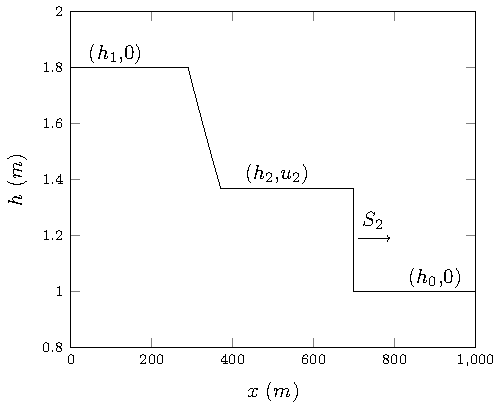
\includegraphics[width=6cm]{../Pics/Edit/SWWlabel.pdf}
		\caption{SWW analytic solution to dam break problem.}
		\label{fig:SWWval}
	\end{figure}
	
\end{frame}
\begin{frame}
	%Besides the obvious oscillations we get due to dispersion it would also be interesting to know 1. if any other properties of the undular bore are the same without dispersion and 2. whether the solution of the Serre equations avergaed over the oscilations is the same as the SWWE
	
	\begin{subequations}
		\begin{gather*}
		h_2 = \frac{h_0}{2} \left[\sqrt{1 + 8 \left(\frac{2h_2}{h_2 - h_0}\frac{\sqrt{gh_1} - \sqrt{gh_2}}{\sqrt{gh_0}}\right)^2} - 1\right],
		\label{eq:h2def}
		\end{gather*}
		\begin{gather*}
		u_2 = 2\left(\sqrt{gh_1} - \sqrt{gh_2}\right),
		\label{eq:u2def}
		\end{gather*}
		\begin{gather*}
		S_2 = \frac{h_2 u_2}{h_2 - h_0}.
		\label{eq:S2def}
		\end{gather*}
		
	\end{subequations}
	
\end{frame}


\begin{frame}{El and Grimshaws Whitham Modulation}
	%Most of the El paper is actually dedicated to applying Whitham modulation to the Serre equations and getting some analytic results for the behaviour of an unudular bore that way, this was the papers main result, it gives a relation for the leading wave amoplitude given the dam break heights as well as the leading wave speed. (Assumptions:)
	
		\begin{figure}
			\centering
			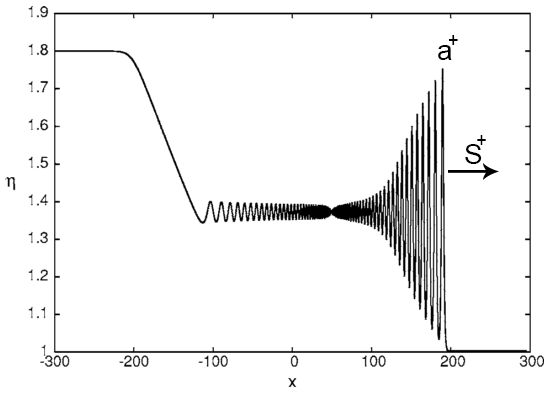
\includegraphics[width=7cm]{../Pics/Diagrams/ElValsDiagram.png}
			\caption{Whitham modulation values demonstrated on El and Grimshaws numerical results}
			\label{fig:ELmod}
		\end{figure}
		
	
\end{frame}

\begin{frame}
	\begin{subequations}
		\begin{gather*}
		\frac{\Delta}{\left(a^+ + 1\right)^{1/4}} - \left(\frac{3}{4 -  \sqrt{a^+ + 1}}\right)^{21/10} \left(\frac{2}{1 + \sqrt{a^+ + 1}}\right)^{2/5} = 0
		\label{eq:aplusdef}
		\end{gather*}
		\begin{gather*}
		S^+ = \sqrt{g \left(a^+ + 1\right)}
		\label{eq:splusdef}
		\end{gather*}
	\end{subequations}
	where $\Delta = \frac{h_1 - h_0}{h_0}$. Appropriate when  $\Delta \le 1.43$.
	
\end{frame}

\section{Numerical Results}
\begin{frame}{Findings}
	Literature
	\begin{itemize}
		\item El and Grimshaws numerical and analytic results supported, but do not give the full picture.
		\item Le M\'{e}tayers first order scheme is too diffusive.
		\item Mistotakis initial conditions were not sufficiently steep.
		\item SWW analytic solution is a useful guide for the mean behaviour of the fluid.
	\end{itemize}	
\end{frame}


\subsection{Method}
\begin{frame}{Methods}
%We have 3 methods using the same idea as the Hank paper but for second and third order as well as first order.

%Also have 2 methods like Els results, one replicating it and one replacing the lax wendroff method for the continuity equation with a naive second orer centered FD approximation

%well validated
Le M\'{e}tayer methods.
\begin{itemize}
	\item First order
	\item Second order
	\item Third order
\end{itemize}

Finite Difference Method
\begin{itemize}
	\item El and Grimshaws
\end{itemize}

\end{frame}

\begin{frame}{Initial Conditions}

%We also do replicate the dam break problem used by Hank and El that is 1.8m and 1m, our three Hank like methods can handle discontinuities, while our El like methods cannot so we employ smoothing of the initial conditions for various alphas and various resolutions

%this also allows us to use the same smoothing as Dutyhk

\begin{figure}
	\centering
	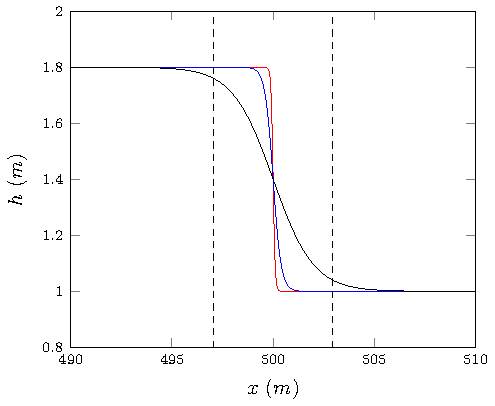
\includegraphics[width=6cm]{../Pics/Edit/ICall.pdf}
	\caption{Initial Conditions where $\beta = 0.294$ ({\color{red} \solidrule}), $\beta = 1.17778$ ({\color{blue} \solidrule}), $\beta = 5.8888$ ({\color{black} \solidrule}) with reference $\beta$ interval({\color{black} \dashedrule}).}
	\label{fig:IC}
\end{figure}

\end{frame}


\subsection{Water Profile}
\begin{frame}{$\beta = 5.8888$}
%This is the smoothing Dutyhk and we replicated their results for all our methods and all our resolutions,
\begin{figure}
\begin{tikzpicture}
\draw [dashed,orange] (27.5,-19.4) -- (30.5,-17.9);

\draw [dashed,orange] (27.5,-20.35) -- (30.5,-21.7);
\node[anchor=east] at (30,-20) {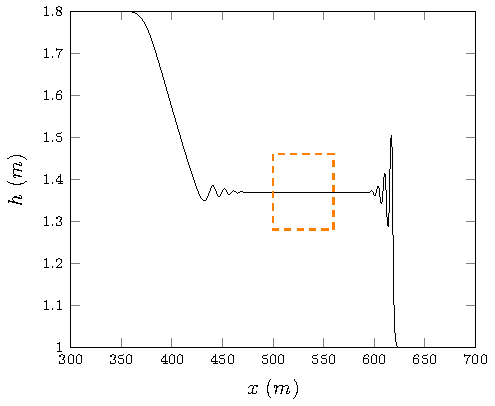
\includegraphics[width=5.4cm]{../Pics/Edit/dxTo0/alpha6/1/Collect/1d.pdf}};
\node[anchor=west] at (30,-20) {\includegraphics[width=5.4cm]{../Pics/Edit/dxTo0/alpha6/2/Collect/1d.pdf}};
\end{tikzpicture}
\caption{Numerical results of third order Le M\'{e}tayer method at $30s$ with  $ \Delta x  = \frac{10}{2^4}$ ({\color{black} \solidrule}).}
\end{figure}
\end{frame}

\begin{frame}
	%This is the smoothing Dutyhk and we replicated their results for all our methods and all our resolutions,
	\begin{figure}
		\begin{tikzpicture}
		\draw [dashed,orange] (27.5,-19.4) -- (30.5,-17.9);
		
		\draw [dashed,orange] (27.5,-20.35) -- (30.5,-21.7);
		\node[anchor=east] at (30,-20) {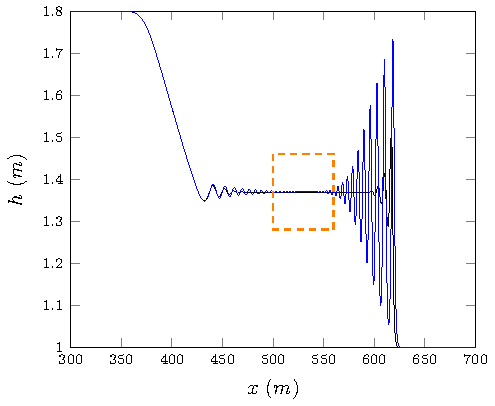
\includegraphics[width=5.4cm]{../Pics/Edit/dxTo0/alpha6/1/Collect/2d.pdf}};
		\node[anchor=west] at (30,-20) {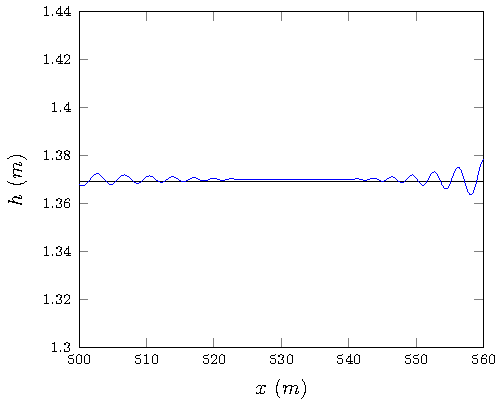
\includegraphics[width=5.4cm]{../Pics/Edit/dxTo0/alpha6/2/Collect/2d.pdf}};
		\end{tikzpicture}
		\caption{Numerical results of third order Le M\'{e}tayer method at $30s$ with a $ \Delta x$ of $\frac{10}{2^4}$ ({\color{black} \solidrule}) and $\frac{10}{2^7}$ ({\color{blue} \solidrule}).}
	\end{figure}
\end{frame}

\begin{frame}
	%This is the smoothing Dutyhk and we replicated their results for all our methods and all our resolutions,
	\begin{figure}
		\begin{tikzpicture}
		\draw [dashed,orange] (27.5,-19.4) -- (30.5,-17.9);
		
		\draw [dashed,orange] (27.5,-20.35) -- (30.5,-21.7);
		\node[anchor=east] at (30,-20) {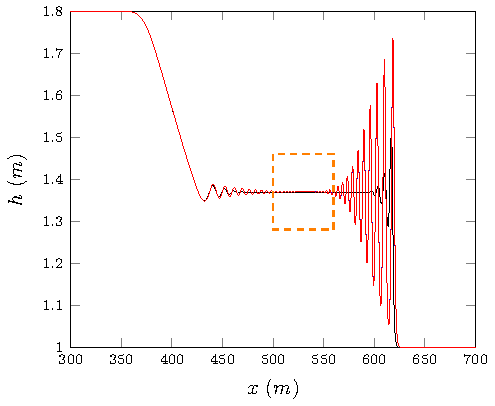
\includegraphics[width=5.4cm]{../Pics/Edit/dxTo0/alpha6/1/Collect/all.pdf}};
		\node[anchor=west] at (30,-20) {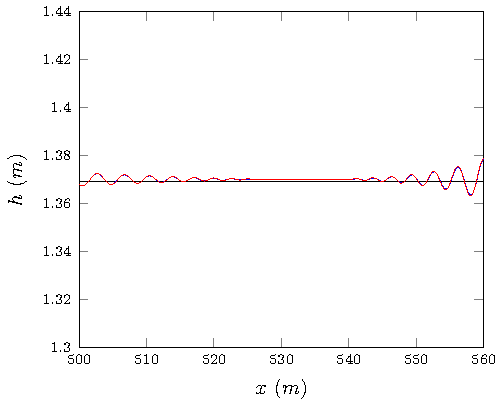
\includegraphics[width=5.4cm]{../Pics/Edit/dxTo0/alpha6/2/Collect/all.pdf}};
		\end{tikzpicture}
		\caption{Numerical results of third order Le M\'{e}tayer method at $30s$ with a $ \Delta x$ of $\frac{10}{2^4}$ ({\color{black} \solidrule}) , $\frac{10}{2^7}$ ({\color{blue} \solidrule}) and $\frac{10}{2^{10}}$ ({\color{red} \solidrule}).}
	\end{figure}
\end{frame}

\begin{frame}{$\beta = 1.17778$}
%Using a steeper problem we are able to replicate Els results with all methods given sufficient resolution (? first order?)

%we find that solving this dam break problem is very sensitive to both the diffusivity of the scheme (first order) as well as the smoothness of the initial conditions

	\begin{figure}
		\begin{tikzpicture}
		\draw [dashed,orange] (27.5,-19.4) -- (30.5,-17.9);
		
		\draw [dashed,orange] (27.5,-20.35) -- (30.5,-21.7);
		\node[anchor=east] at (30,-20) {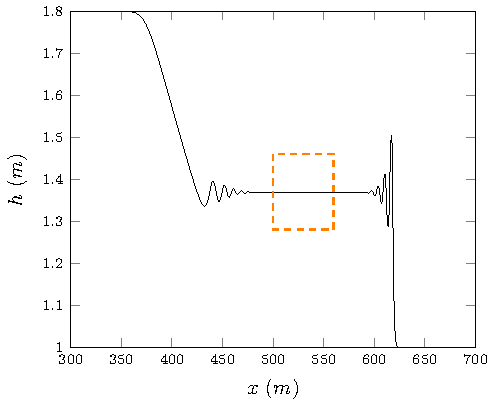
\includegraphics[width=5.4cm]{../Pics/Edit/dxTo0/alpha9/1/Collect/1d.pdf}};
		\node[anchor=west] at (30,-20) {\includegraphics[width=5.4cm]{../Pics/Edit/dxTo0/alpha9/2/Collect/1d.pdf}};
		\end{tikzpicture}
		\caption{Numerical results of third order Le M\'{e}tayer method at $30s$ with a $ \Delta x$ of $\frac{10}{2^4}$ ({\color{black} \solidrule}).}
	\end{figure}


\end{frame}

\begin{frame}
	
	\begin{figure}
		\begin{tikzpicture}
		\draw [dashed,orange] (27.5,-19.4) -- (30.5,-17.9);
		
		\draw [dashed,orange] (27.5,-20.35) -- (30.5,-21.7);
		\node[anchor=east] at (30,-20) {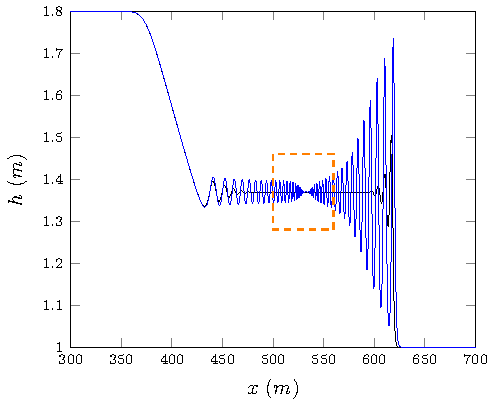
\includegraphics[width=5.4cm]{../Pics/Edit/dxTo0/alpha9/1/Collect/2d.pdf}};
		\node[anchor=west] at (30,-20) {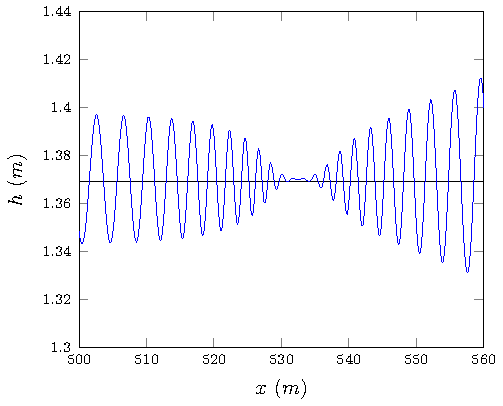
\includegraphics[width=5.4cm]{../Pics/Edit/dxTo0/alpha9/2/Collect/2d.pdf}};
		\end{tikzpicture}
		\caption{Numerical results of third order Le M\'{e}tayer method at $30s$ with a $ \Delta x$ of $\frac{10}{2^4}$ ({\color{black} \solidrule}) and $\frac{10}{2^7}$ ({\color{blue} \solidrule}).}
	\end{figure}
	
	
\end{frame}

\begin{frame}
	
	\begin{figure}
		\begin{tikzpicture}
		\draw [dashed,orange] (27.5,-19.4) -- (30.5,-17.9);
		
		\draw [dashed,orange] (27.5,-20.35) -- (30.5,-21.7);
		\node[anchor=east] at (30,-20) {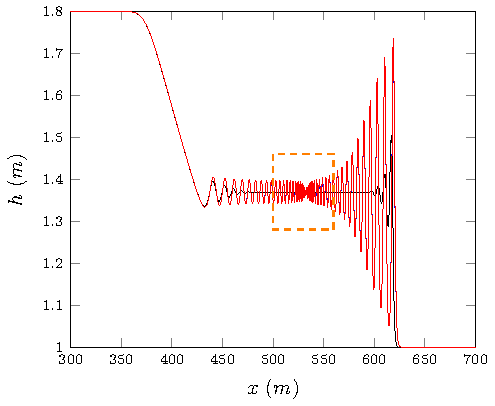
\includegraphics[width=5.4cm]{../Pics/Edit/dxTo0/alpha9/1/Collect/all.pdf}};
		\node[anchor=west] at (30,-20) {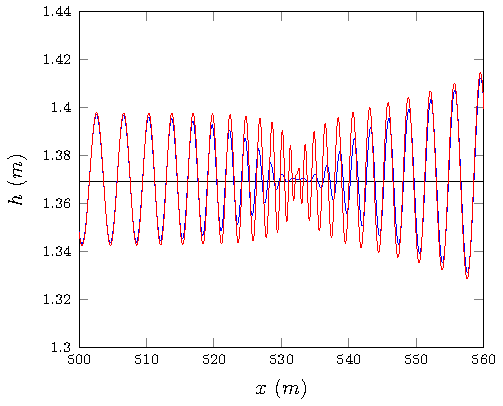
\includegraphics[width=5.4cm]{../Pics/Edit/dxTo0/alpha9/2/Collect/all.pdf}};
		\end{tikzpicture}
		\caption{Numerical results of third order Le M\'{e}tayer method at $30s$ with a $ \Delta x$ of $\frac{10}{2^4}$ ({\color{black} \solidrule}), $\frac{10}{2^7}$ ({\color{blue} \solidrule}) and $\frac{10}{2^{10}}$ ({\color{red} \solidrule}).}
	\end{figure}
	
	
\end{frame}

\begin{frame}{Dispersion Relation}
	%Linearising the Serre equations one obtains
	%\begin{equation}
	%\frac{\partial h_1}{\partial t} + u_0\frac{\partial h_1}{\partial x} + h_0\frac{\partial u_1}{\partial x} = 0 
	%\end{equation} 
	%\begin{equation}
	%\frac{\partial u_1}{\partial t} + g\frac{\partial h_1}{\partial x} + u_0\frac{\partial u_1}{\partial x} - \frac{h_0^2}{3}\left(u_0\frac{\partial^3 u_1}{\partial x^3} + \frac{\partial^3 u_1}{\partial x^2 \partial t}  \right) = 0 
	%\end{equation} 
	%and setting $h_1(x,t) = H e^{i(kx - \omega t)}$ and $u_1(x,t) = U e^{i(kx - \omega t)}$
	The dispersion relation for the linearised Serre equations is 
	
	\[\omega =u_0 k \pm k\sqrt{gh_0} \sqrt{\frac{3}{h_0^2 k^2 + 3}} \]
	
	Thus the phase speed is
	
	\[\upsilon_p =u_0 \pm \sqrt{gh_0} \sqrt{\frac{3}{h_0^2 k^2 + 3}} \]
	
	Taking $k \rightarrow 0$ we see $\upsilon_p  \rightarrow u_0 \pm \sqrt{gh_0} $
	
	Taking $k \rightarrow \infty$ we see $\upsilon_p  \rightarrow u_0 $
	
\end{frame}

\begin{frame}{Contact Discontinuity}
	
		\begin{figure}
			\begin{tikzpicture}
			\node[] at (30,-20) {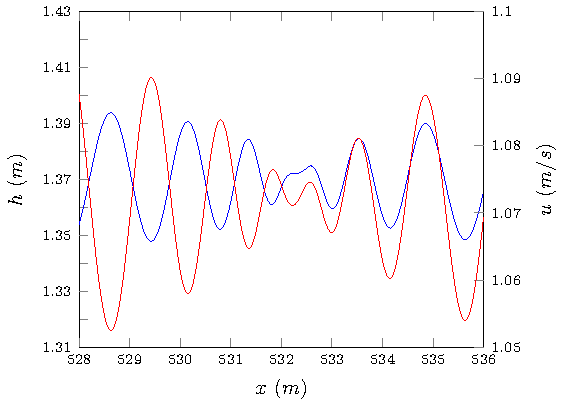
\includegraphics[width=6.5cm]{../Pics/Edit/uhCD.pdf}};
			\end{tikzpicture}
			\caption{plot of $h$ ({\color{blue} \solidrule}) and $u$ ({\color{red} \solidrule}) around contact discontinuity for third order Le M\'{e}tayer method with $\Delta x = \frac{10}{2^{10}}$ at $30s$.}
		\end{figure}
	
\end{frame}



\begin{frame}{$\beta = 0.294$}
%Using an even steeper problem we are able to see new results that so far have not been reported, we see this for all methods with sufficient resolution

%surprising, but there are some ncie things for isntance since we have both dispersive and diffusive schemes we know that the solution is between these two, so in particular this bump is not going to blow up and ruin the scheme


	\begin{figure}
		\begin{tikzpicture}
		\draw [dashed,orange] (27.5,-19.4) -- (30.5,-17.9);
		
		\draw [dashed,orange] (27.5,-20.35) -- (30.5,-21.7);
		\node[anchor=east] at (30,-20) {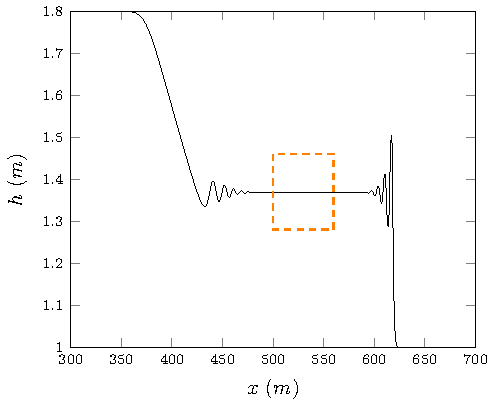
\includegraphics[width=5.4cm]{../Pics/Edit/dxTo0/alpha12/1/Collect/1d.pdf}};
		\node[anchor=west] at (30,-20) {\includegraphics[width=5.4cm]{../Pics/Edit/dxTo0/alpha12/2/Collect/1d.pdf}};
		\end{tikzpicture}
		\caption{Numerical results of third order Le M\'{e}tayer method at $30s$ with a $ \Delta x$ of $\frac{10}{2^4}$ ({\color{black} \solidrule}).}
	\end{figure}

\end{frame}

\begin{frame}

	\begin{figure}
		\begin{tikzpicture}
		\draw [dashed,orange] (27.5,-19.4) -- (30.5,-17.9);
		
		\draw [dashed,orange] (27.5,-20.35) -- (30.5,-21.7);
		\node[anchor=east] at (30,-20) {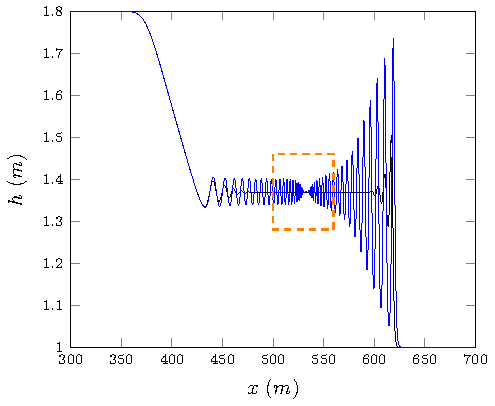
\includegraphics[width=5.4cm]{../Pics/Edit/dxTo0/alpha12/1/Collect/2d.pdf}};
		\node[anchor=west] at (30,-20) {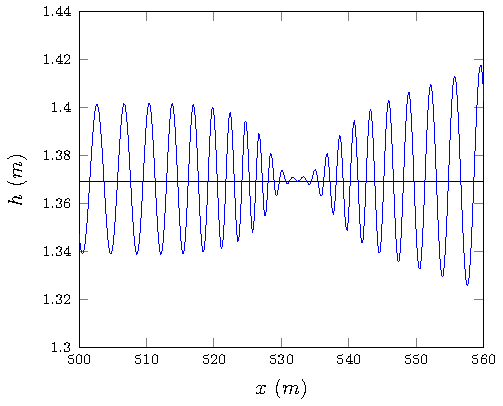
\includegraphics[width=5.4cm]{../Pics/Edit/dxTo0/alpha12/2/Collect/2d.pdf}};
		\end{tikzpicture}
		\caption{Numerical results of third order Le M\'{e}tayer method at $30s$ with a $ \Delta x$ of $\frac{10}{2^4}$ ({\color{black} \solidrule}) and $\frac{10}{2^7}$ ({\color{blue} \solidrule}).}
	\end{figure}
	
\end{frame}

\begin{frame}
	
	\begin{figure}
		\begin{tikzpicture}
		\draw [dashed,orange] (27.5,-19.4) -- (30.5,-17.9);
		
		\draw [dashed,orange] (27.5,-20.35) -- (30.5,-21.7);
		\node[anchor=east] at (30,-20) {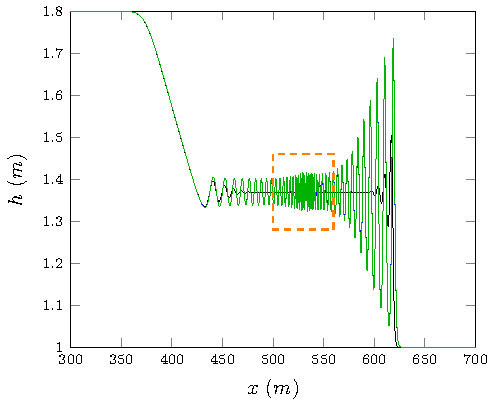
\includegraphics[width=5.4cm]{../Pics/Edit/dxTo0/alpha12/1/Collect/3d.pdf}};
		\node[anchor=west] at (30,-20) {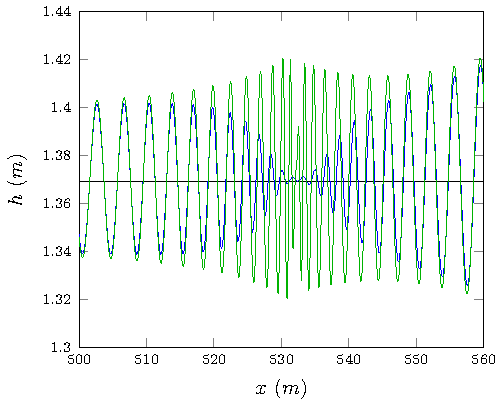
\includegraphics[width=5.4cm]{../Pics/Edit/dxTo0/alpha12/2/Collect/3d.pdf}};
		\end{tikzpicture}
		\caption{Numerical results of third order Le M\'{e}tayer method at $30s$ with a $ \Delta x$ of $\frac{10}{2^4}$ ({\color{black} \solidrule}) , $\frac{10}{2^7}$ ({\color{blue} \solidrule}) and $\frac{10}{2^9}$ ({\color{green!70!black} \solidrule}).}
	\end{figure}
	
\end{frame}

\begin{frame}
	
	\begin{figure}
		\begin{tikzpicture}
		\draw [dashed,orange] (27.5,-19.4) -- (30.5,-17.9);
		
		\draw [dashed,orange] (27.5,-20.35) -- (30.5,-21.7);
		\node[anchor=east] at (30,-20) {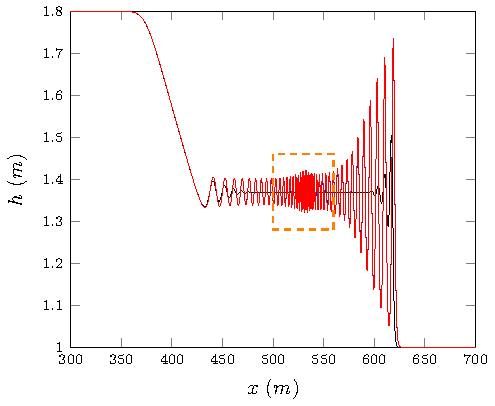
\includegraphics[width=5.4cm]{../Pics/Edit/dxTo0/alpha12/1/Collect/all.pdf}};
		\node[anchor=west] at (30,-20) {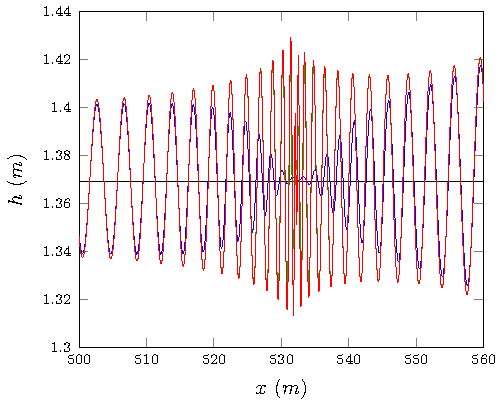
\includegraphics[width=5.4cm]{../Pics/Edit/dxTo0/alpha12/2/Collect/all.pdf}};
		\end{tikzpicture}
		\caption{Numerical results of third order Le M\'{e}tayer method at $30s$ with a $ \Delta x$ of $\frac{10}{2^4}$ ({\color{black} \solidrule}) , $\frac{10}{2^7}$ ({\color{blue} \solidrule}) , $\frac{10}{2^9}$ ({\color{green!70!black} \solidrule}) and $\frac{10}{2^{10}}$ ({\color{red} \solidrule}).}
	\end{figure}
	
\end{frame}


\begin{frame}{$\beta = 0.294$ Various Models}
	\begin{figure}
		\begin{tikzpicture}
		\draw [dashed,orange] (27.5,-19.4) -- (30.5,-17.9);
		
		\draw [dashed,orange] (27.5,-20.35) -- (30.5,-21.7);
		\node[anchor=east] at (30,-20) {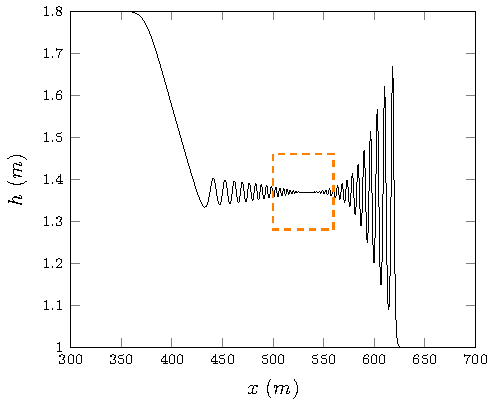
\includegraphics[width=5.4cm]{../Pics/Edit/ManyModels/1/Collect/1d.pdf}};
		\node[anchor=west] at (30,-20) {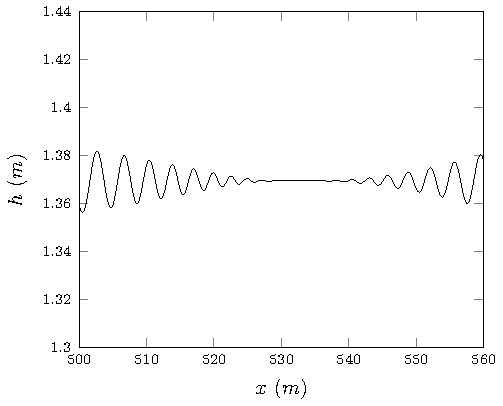
\includegraphics[width=5.4cm]{../Pics/Edit/ManyModels/2/Collect/1d.pdf}};
		\end{tikzpicture}
		\caption{Numerical results at $30s$ with a $ \Delta x = \frac{10}{2^{10}}$ for the first order({\color{black} \solidrule}) Le M\'{e}tayer method.}
	\end{figure}	

		%\caption{Numerical results at $30s$ for Le M\'{e}tayer methods of first ({\color{black} \solidrule}) , second ({\color{yellow!70!black} \solidrule}) and third-order ({\color{violet!70!white} \solidrule}) as well Els method ({\color{red} \solidrule}).}
	
\end{frame}

\begin{frame}
	\begin{figure}
		\begin{tikzpicture}
		\draw [dashed,orange] (27.5,-19.4) -- (30.5,-17.9);
		
		\draw [dashed,orange] (27.5,-20.35) -- (30.5,-21.7);
		\node[anchor=east] at (30,-20) {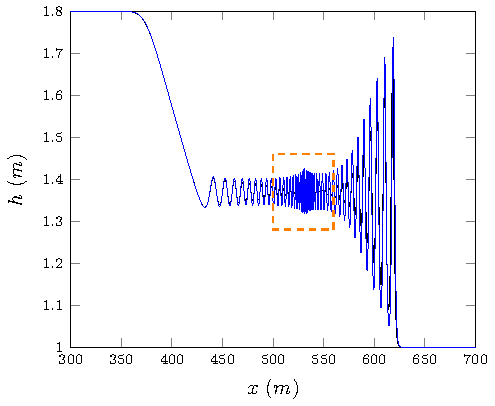
\includegraphics[width=5.4cm]{../Pics/Edit/ManyModels/1/Collect/2d.pdf}};
		\node[anchor=west] at (30,-20) {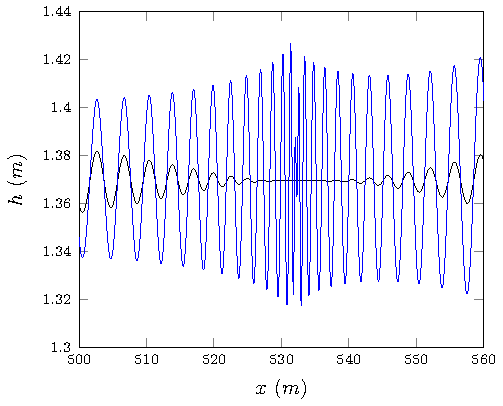
\includegraphics[width=5.4cm]{../Pics/Edit/ManyModels/2/Collect/2d.pdf}};
		\end{tikzpicture}
		\caption{Numerical results at $30s$ with a $ \Delta x = \frac{10}{2^{10}}$ for the first order ({\color{black} \solidrule}) and second order ({\color{blue} \solidrule}) Le M\'{e}tayer method.}
	\end{figure}		
\end{frame}

\begin{frame}
	\begin{figure}
		\begin{tikzpicture}
		\draw [dashed,orange] (27.5,-19.4) -- (30.5,-17.9);
		
		\draw [dashed,orange] (27.5,-20.35) -- (30.5,-21.7);
		\node[anchor=east] at (30,-20) {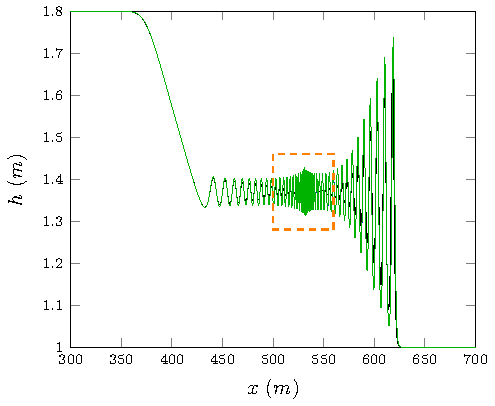
\includegraphics[width=5.4cm]{../Pics/Edit/ManyModels/1/Collect/3d.pdf}};
		\node[anchor=west] at (30,-20) {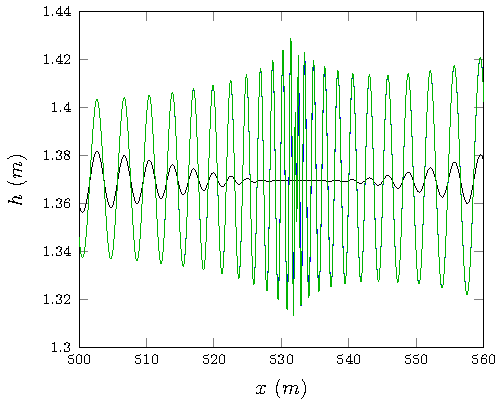
\includegraphics[width=5.4cm]{../Pics/Edit/ManyModels/2/Collect/3d.pdf}};
		\end{tikzpicture}
		\caption{Numerical results at $30s$ with a $ \Delta x = \frac{10}{2^{10}}$ for the first order ({\color{black} \solidrule}), second order ({\color{blue} \solidrule})  and third order ({\color{green!70!black} \solidrule}) Le M\'{e}tayer method.}
	\end{figure}		
\end{frame}

\begin{frame}
	\begin{figure}
		\begin{tikzpicture}
		\draw [dashed,orange] (27.5,-19.4) -- (30.5,-17.9);
		
		\draw [dashed,orange] (27.5,-20.35) -- (30.5,-21.7);
		\node[anchor=east] at (30,-20) {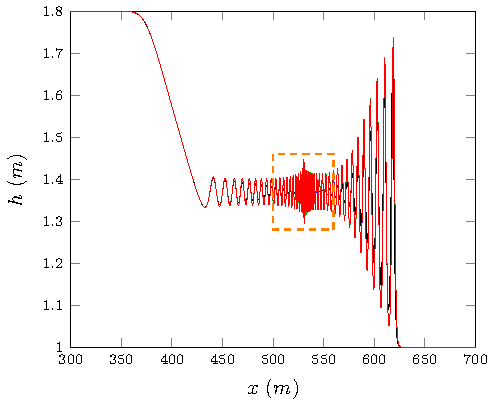
\includegraphics[width=5.4cm]{../Pics/Edit/ManyModels/1/Collect/all.pdf}};
		\node[anchor=west] at (30,-20) {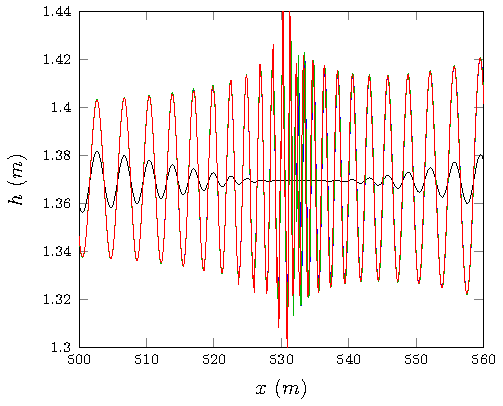
\includegraphics[width=5.4cm]{../Pics/Edit/ManyModels/2/Collect/all.pdf}};
		\end{tikzpicture}
		\caption{Numerical results at $30s$ with a $ \Delta x = \frac{10}{2^{10}}$ for the first order ({\color{black} \solidrule}), second order ({\color{blue} \solidrule})  and third order ({\color{green!70!black} \solidrule}) Le M\'{e}tayer method and El and Grimshaws method ({\color{red} \solidrule}).}
	\end{figure}		
\end{frame}


\begin{frame}{$\beta = 0.294$ Long Time}
%We also see that allowing the scheme to run longer this situation reverts back to the contact discontinutyi and then the Hank results. 

	\begin{figure}
		\centering
		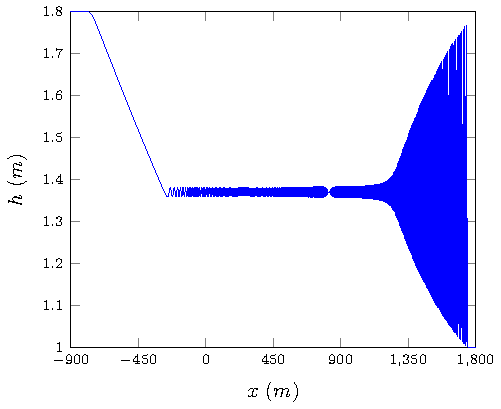
\includegraphics[width=6cm]{../Pics/MyPlots/numsols/300s/0-figure0.pdf}
		\label{fig:numsolsalpha10LT}
		\caption{Numerical results at $300s$ with $\Delta x =10 / 2^9$ for third-order Le M\'{e}tayer Method.}
	\end{figure}



\end{frame}

\begin{frame}{}
	\begin{figure}
		\centering
		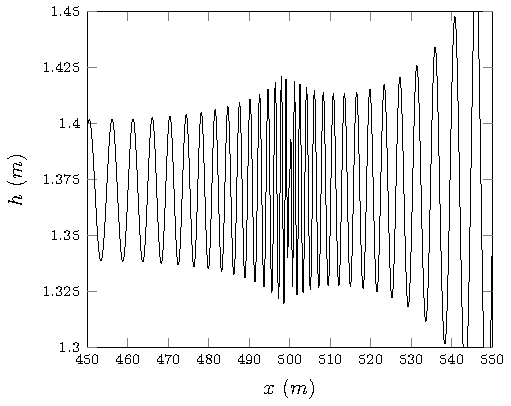
\includegraphics[width=7cm]{../Pics/Edit/DBOT/Collect/1d.pdf}
		\caption{Translated numerical results with $\Delta x =10 / 2^9$ at $30s$ ({\color{black} \solidrule}) using third order Le M\'{e}tayer method.}
	\end{figure}
	
\end{frame}
\begin{frame}{}
	\begin{figure}
		\centering
		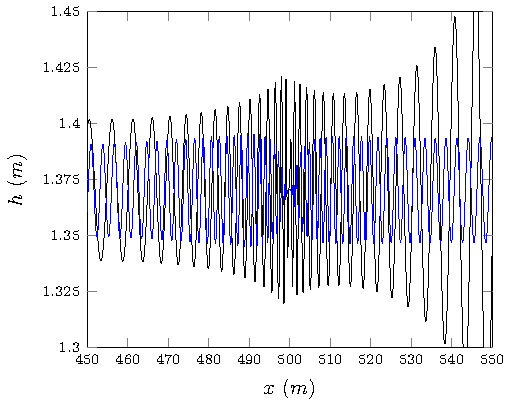
\includegraphics[width=7cm]{../Pics/Edit/DBOT/Collect/2.pdf}
		\caption{Translated numerical results with $\Delta x =10 / 2^9$ at $30s$ ({\color{black} \solidrule}) , $100s$ ({\color{blue} \solidrule}) using third order Le M\'{e}tayer method. }
	\end{figure}
	
\end{frame}

\begin{frame}{}
	\begin{figure}
		\centering
		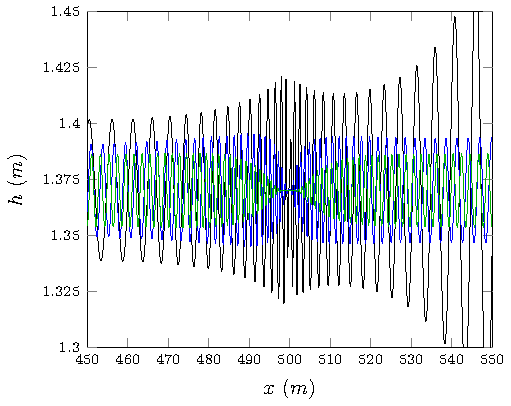
\includegraphics[width=7cm]{../Pics/Edit/DBOT/Collect/3d.pdf}
		\caption{Translated numerical results with $\Delta x =10 / 2^9$ at $30s$ ({\color{black} \solidrule}) , $100s$ ({\color{blue} \solidrule}) , $200s$ ({\color{green!70!black} \solidrule}) using third order Le M\'{e}tayer method.}
	\end{figure}
	
\end{frame}

\begin{frame}{}
	\begin{figure}
		\centering
		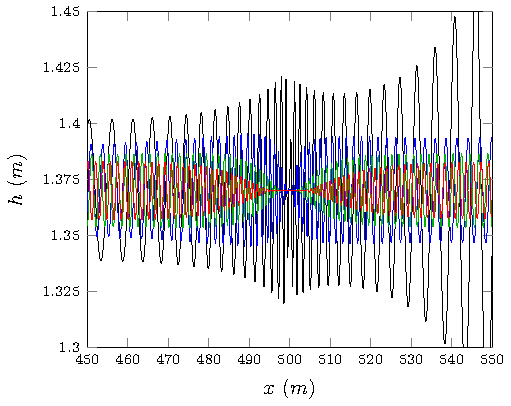
\includegraphics[width=7cm]{../Pics/Edit/DBOT/Collect/all.pdf}
		\caption{Translated numerical results with $\Delta x =10 / 2^9$ at $30s$ ({\color{black} \solidrule}) , $100s$ ({\color{blue} \solidrule}) , $200s$ ({\color{green!70!black} \solidrule}) and $300s$ ({\color{red} \solidrule}) using third order Le M\'{e}tayer method.}
	\end{figure}
	
\end{frame}


\subsection{SWWE Solution Comparison}
\begin{frame}{}
	\begin{figure}
		\centering
		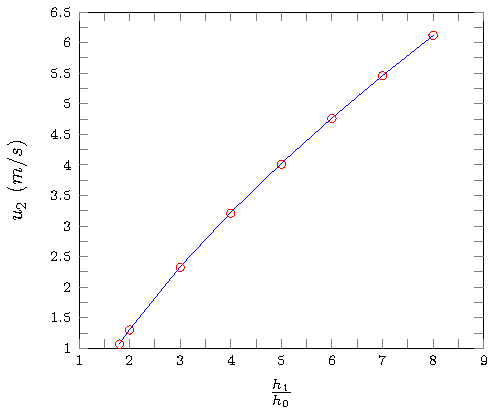
\includegraphics[width=6cm]{../Pics/Edit/u2fordifferentAR.pdf}
		\label{fig:SWWcomp}
		\caption{compares $u_2$ ({\color{blue} \solidrule }) to the average speed of the contact discontinuity ({\color{red} $\circ$}) for third order Le M\'{e}tayer method with $\Delta x = \frac{10}{2^{9}}$ at $300s$. }
	\end{figure}
\end{frame}

\begin{frame}{}
		\begin{figure}
			\centering
			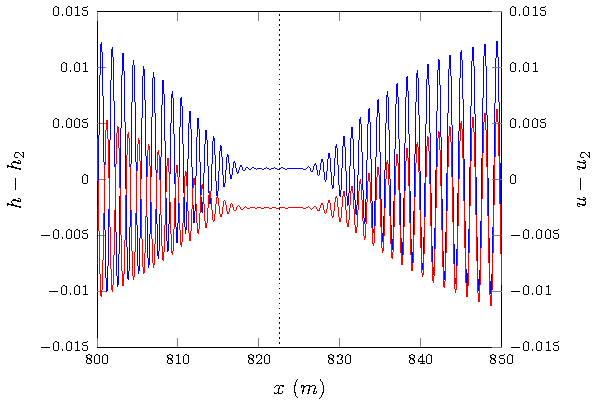
\includegraphics[width=7cm]{../Pics/Edit/uhlongtime.pdf}
			\label{fig:SWWcompuh}
			\caption{plot of $h - h_2$ ({\color{blue} \solidrule}) and $u - u_2$ ({\color{red} \solidrule}) with $x_2$ ({\color{black} \dotrule{0.05\textwidth} }) for third order Le M\'{e}tayer method with $\Delta x = \frac{10}{2^{9}}$ at $300s$.}
		\end{figure}
\end{frame}

\begin{frame}{}
	\begin{figure}
		\centering
		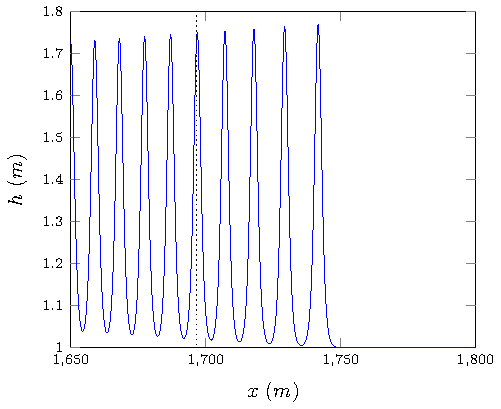
\includegraphics[width=6cm]{../Pics/Edit/S2.pdf}
		\label{fig:SWWcompSplus}
		\caption{Plot comparing numerical results for shock front of the Serre equations to $S_2$  for third order Le M\'{e}tayer method with $\Delta x = \frac{10}{2^{9}}$ at $300s$.}	
	\end{figure}
	
\end{frame}

\subsection{Els Analytic Comparison}


\begin{frame}{}
	\begin{figure}
		\centering
		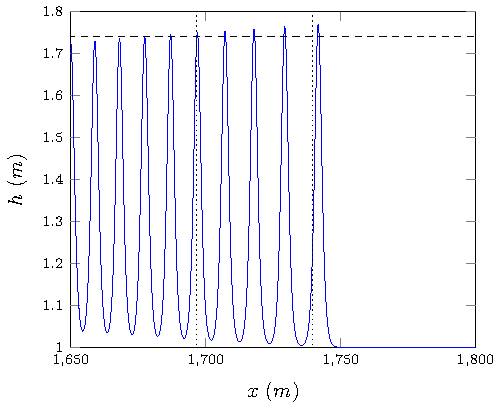
\includegraphics[width=6cm]{../Pics/Edit/Splus.pdf}
		\label{fig:ELcompSplus}
		\caption{Plot comparing numerical results for shock front of the Serre equations to $S^+$ ({\color{black} \dotrule{0.05\textwidth} }), $S_2$({\color{black} \dotrule{0.05\textwidth} })and $a^+$ ({\color{black} \dashedrule }) for third order Le M\'{e}tayer method with $\Delta x = \frac{10}{2^{9}}$ at $300s$.}	
	\end{figure}
	
\end{frame}

\begin{frame}{}
	\begin{figure}
		\centering
		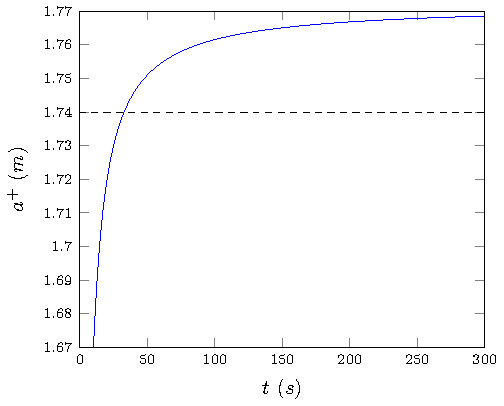
\includegraphics[width=7cm]{../Pics/MyPlots/numsols/300s/a.pdf}
		\caption{Plot of lead oscillation amplitude over time for third order Le M\'{e}tayer method with $\Delta x = \frac{10}{2^{9}}$ at $300s$ with analytic comparison ({\color{black} \dashedrule })}	
		%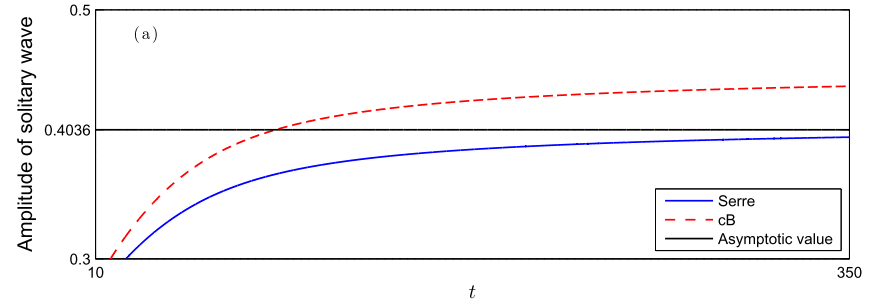
\includegraphics[width=6.5cm]{../Pics/Lit/SmoothDBDutyhkA.png}
		%\caption{Left plot shows how our lead soliton amplitude evolves over time  for third order Le M\'{e}tayer method with $\Delta x = \frac{10}{2^{9}}$ at $300s$ with analytic comparison ({\color{black} \dashedrule }). Right plot shows the same plot from the Mitsokakis paper.}	
		\label{fig:ELcompLIT}
	\end{figure}
	
\end{frame}

\begin{frame}{Conclusions}
	Literature
	\begin{itemize}
		\item Supports Els results
		    \begin{itemize}
		    	\item{Best numerical results for the dam break problem}
		    	\item{$a^+$ seems to underestimate lead oscillation amplitude}
		    	\item{$S^+$ underestimates speed}
		    \end{itemize}
		\item Le M\'{e}tayers first order scheme is too diffusive
		\item Mistotakis initial conditions were not sufficiently steep
		\item SWW analytic solution is a useful guide for the mean bore height $h_2$ (underestimate), mean bore velocity $u_2$ (overestimate) and speed of the bore $S_2$ (underestimate)
	\end{itemize}	
\end{frame}

\begin{frame}[allowframebreaks]{References}
%--------------------------------------------------------------------------------
\bibliography{pres}
\bibliographystyle{apalike}
%--------------------------------------------------------------------------------
\end{frame}

\section{Appendices}
\subsection{Supplementary Plots}
\begin{frame}{Zoom in on $u$ and $h$}
	\begin{figure}
		\centering
		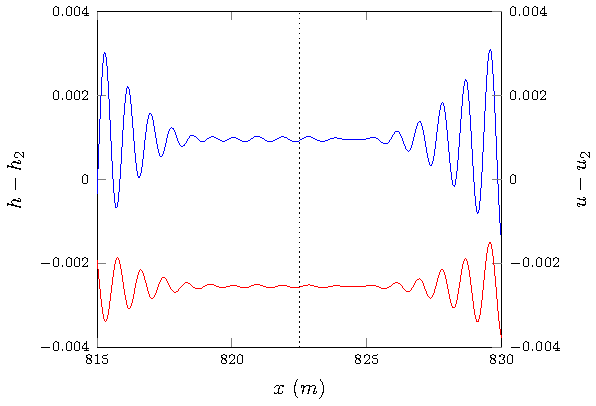
\includegraphics[width=4.6cm]{../Pics/Edit/UHLTZoom.pdf}
		\includegraphics[width=4.6cm]{../Pics/Edit/UHLTSUPERZOOM.pdf}
		\caption{plot of $h - h_2$ ({\color{blue} \solidrule}) and $u - u_2$ ({\color{red} \solidrule}) with $x_2$ ({\color{black} \dotrule{0.05\textwidth} })}
	\end{figure}
\end{frame}

\begin{frame}{Zoom in on all Models}
	\begin{figure}
		\centering
		\includegraphics[width=4.6cm]{../Pics/Edit/ManyModels/Supp/3-figure0.pdf}
		\includegraphics[width=4.6cm]{../Pics/Edit/ManyModels/Supp/4-figure0.pdf}
		\caption{Numerical results at $30s$ with a $ \Delta x = \frac{10}{2^{10}}$ for the first order ({\color{black} \solidrule}), second order ({\color{blue} \solidrule})  and third order ({\color{green!70!black} \solidrule}) Le M\'{e}tayer method and El and Grimshaws method ({\color{red} \solidrule}).}
	\end{figure}
\end{frame}

\subsection{Numerical Method}

\begin{frame}{Serre Equations}
	\begin{subequations}
		\begin{gather*}
		\dfrac{\partial h}{\partial t} + \dfrac{\partial (uh)}{\partial x} = 0,
		\end{gather*}
		\begin{gather*}
		\underbrace{\underbrace{\dfrac{\partial (uh)}{\partial t} + \dfrac{\partial}{\partial x} \left ( u^2h + \dfrac{gh^2}{2}\right )}_{\text{Shallow Water Wave Equations}} + \underbrace{\dfrac{\partial}{\partial x} \left (  \dfrac{h^3}{3} \left [ \dfrac{\partial u }{\partial x} \dfrac{\partial u}{\partial x} -u \dfrac{\partial^2 u}{\partial x^2}  - \dfrac{\partial^2 u}{\partial x \partial t}\right ] \right )}_{\text{Dispersion Terms}} = 0}_{\text{Serre Equations}}
		\end{gather*}
	\end{subequations}
\end{frame}

\begin{frame}{Conservation Law Form}
	New conserved quantity
	\begin{gather}\label{eq:Gdefinition}
	G = uh - h^2 \dfrac{\partial h}{\partial x} \dfrac{\partial u}{\partial x} - \frac{h^3}{3} \dfrac{\partial^2 u}{\partial x^2}.
	\end{gather}
	Reformulated equations
	\begin{subequations}
		\begin{gather}
		\dfrac{\partial h}{\partial t} + \dfrac{\partial (uh)}{\partial x} = 0
		\label{eq:Serrecon_continuity}
		\end{gather}
		\begin{gather}
		\dfrac{\partial G}{\partial t} + \dfrac{\partial}{\partial x}\left(Gu + \dfrac{gh^2}{2} - \dfrac{2h^3}{3}\dfrac{\partial u}{\partial x}\dfrac{\partial u}{\partial x}\right) = 0
		\label{eq:Serrecon_momentum}
		\end{gather}
		\label{eq:Serrecon}
	\end{subequations}
\end{frame}

\begin{frame}{Basic Overview}
	Vector of conserved quantities:
	\[\boldsymbol{U} = 
	\left[
	\begin{array}{c}
	h \\
	G							
	\end{array} \right] \]
	
	Algorithm:
	\[\mathcal{H}\left(\boldsymbol{\bar{U}}^n,\Delta x ,\Delta t \right) = \left\lbrace 
	\begin{array}{c c c} 
	\boldsymbol{U}^n &=& \mathcal{M}\left(\boldsymbol{\bar{U}}^n\right) \\
	\boldsymbol{u}^n &=& \mathcal{A}\left(\boldsymbol{U}^n, \Delta x\right) \\
	\boldsymbol{\bar{U}}^{n+1} &=& \mathcal{L}\left(\boldsymbol{\bar{U}}^{n},\boldsymbol{u}^n, \Delta x ,\Delta t\right)							
	\end{array} \right. .\]
\end{frame}


\end{document}